%%%%%%%%%%%%%%%%%%%%%%%%%%%%%%%%%%%%%%%%%%%%%%%%%%
%%%%%%%%%%%%%%%%%% EXPERIMENTAL %%%%%%%%%%%%%%%%%%
%%%%%%%%%%%%%%%%%%%%%%%%%%%%%%%%%%%%%%%%%%%%%%%%%%
In this section the used chemicals and substrates, experimental procedures and any used 
equipment are described. 
%\td{Also, the long, exhaustive path to the base solution is described}
The experiments can be split into three sections: 
In the first section the base recipe and the base process were sought. 
In the pre-optimisation section the boundaries for the optimisation were investigated. 
And during the third and final step the experiments for the optimisation were performed.
\section{Substrate Preparation}
%\ds{
Five different substrates were used throughout this work: 
microscope glass slides 
\linebreak[4] 
(\cm{2.5}$\times$\cm{7.5})\ds{ from Sigma Aldrich, thinner}, 
squared glass plates (\cm{2.5}\x\cm{2.5})\ds{ from Sigma Aldrich}, 
\gls{ito} glass plates (\cm{2.5}\x\cm{2.5})\ds{ from Sigma Aldrich}, 
\gls{fto} glass plates (\cm{5}\x\cm{5})\ds{ from Sigma Aldrich} and steel foil (10~cm~x~10~cm) provided by Sunplugged GmbH (\url{http://sunplugged.at/)}.
%}
\ds{
Four different substrates were used throughout this work: 
microscope glass slides, \gls{ito} glass plates, \gls{fto} glass plates and steel foil provided by Sunplugged GmbH (\url{http://sunplugged.at/)}.
}
%
Glass was used because of its availability and to measure transmission and reflectance 
spectra. \gls{fto} and \gls{ito} were used in order to have a conducting substrate, which
is needed to measure the conductivity of the applied layer and for \gls{sem} micrographs.
The glass slides and \gls{fto} were scored with a diamond scribe \ds{\td{(diamond scratcher/scraper)} }and broken with a running plier into pieces of dimensions \cm{2.5}\x\cm{2.5}.
The steel foil was cut with a foil cutter into squares of the same dimensions. 
%, a cutter knife (repeatedly), a paper cutter or a scissors (ordered by increasing curvature of resulting plates).
All substrates were cleaned in three steps before usage:
\begin{enumerate}
	\item \minutes{15} in \ml{50} \gls{water} and \ml{1} of Hellmanex III alkaline concentrate in a sonic bath
	\item \minutes{15} in \gls{water} in a sonic bath
	\item \minutes{15} in \gls{ipo} in a sonic bath 
\end{enumerate}
After the last cleaning step, the samples were blown dry with dry \gls{n2} gas and kept in a clean plastic container until the doctor blading step.

%%%%%%%%%%%%%%%%%%%%%%%%%%%%%%%%%%%%%%%%%%%%%%%%%%%%%%%%%%%%%%%%%%%%%%%%%%%%%%%%%%%%%%%%
%%%%%%%%%%%%%%%%%%%%%%%%%%%%%%%%%%%%%%%%%%%%%%%%%%%%%%%%%%%%%%%%%%%%%%%%%%%%%%%%%%%%%%%%
\section{Solutions}\label{sec:exp-sol}
All recipes for solutions can be divided into two categories:
the first recipe - adopted from Anwar~et~al.~\cite{Anwar2017} - was based on \gls{zrpro} in \gls{acac} and \gls{water} (aquatic solution).
The second recipe - adopted from Hu~et~al.~\cite{Hu2016} - was based on \gls{zrpro} in \gls{buoh} (buthanolic solution).

\begin{figure}[htb]
	\centering
	\begin{subfigure}{0.49\textwidth}
		\centering
		\includegraphics[height=0.8\textwidth]{Pics/sol-aq.png}
		\label{fig:sol-aq}
		\caption{Aquatic solution}
	\end{subfigure}
	\begin{subfigure}{0.49\textwidth}
		\centering
		\includegraphics[height=0.8\textwidth]{Pics/sol-bu.png}
		\label{fig:sol-bu}
		\caption{Buthanolic solution}
	\end{subfigure}
	\label{fig:sol}
	\caption{Aquatic and buthanolic solution with magnetic stirring bars in beaker glass sealed with Parafilm} 
\end{figure}

%%%%%%%%%%%%%%%%%%%%%%%%%%%%%%%%%%%%%%%%%%%%%%%%%%%%%%%%%%%%%%%%%%%%%%%%%%%%%%%%%%%%%%%%
%%%%%%%%%%%%%%%%%%%%%%%%%%%%%%%%%%%%%%%%%%%%%%%%%%%%%%%%%%%%%%%%%%%%%%%%%%%%%%%%%%%%%%%%
\subsection{Aquatic solution}\label{sec:exp-sol-aq}
\gls{zrpro} was added to \gls{acac} while stirring and in a separate vessel \gls{water} 
(including any optional additives such as \gls{sds}, \gls{hcl}, \gls{h2so4} or \gls{naoh}) 
was added to \gls{ipo} and both were stirred for one hour. 
These additives were added to influence pH and surface tension with the goal to influence the resulting layer. % \td{see Parvulescu2015}
The \gls{water}-\gls{ipo} mixture was added to the other solution and stirred over night. 
The exact volumes can be taken from table~\ref{tab:rec1}.
Unfortunately, this solution failed to produce anything near homogeneous layers. 
Thus, an alternative solution was found.
%\td{At this point in time everything was doctor bladed by hand. The hight was varied (with tape).}
\begin{table}[h]
	\centering
	\caption{Compositions of different aquatic solutions}
	\label{tab:rec1}
	\begin{tabular}{llllllll}
		\hline
		recipe				&1		&2		&3		&4		&5		&6		&7\\
		\hline
		\gls{zrpro} [\ml{}]	&8		&8		&8		&8		&8		&8		&8\\
		\gls{acac}  [\ml{}]	&8		&8		&8		&8		&8		&8		&8\\
		\gls{ipo}   [\ml{}]	&2		&2		&2		&2		&2		&2		&2\\
		\gls{water} [\ml{}]	&2.6	&2.6	&2.5	&2~		&2		&2		&2\\
		\gls{sds}   [\mg{}]	&-		&5.9	&-		&-		&-		&-		&-\\
		\gls{hcl}   [\ml{}]	&-		&-		&-		&-		&0.5	&-		&-\\
		\gls{h2so4} [\ml{}]	&-		&-		&-		&-		&-		&0.5	&-\\
		\gls{naoh}  [\ml{}] &-		&-		&-		&-		&-		&-		&0.5\\
		\hline
	\end{tabular}
\end{table}
%
%%%%%%%%%%%%%%%%%%%%%%%%%%%%%%%%%%%%%%%%%%%%%%%%%%%%%%%%%%%%%%%%%%%%%%%%%%%%%%%%%%%%%%%%
%%%%%%%%%%%%%%%%%%%%%%%%%%%%%%%%%%%%%%%%%%%%%%%%%%%%%%%%%%%%%%%%%%%%%%%%%%%%%%%%%%%%%%%%
\subsection{Buthanolic solution}\label{sec:exp-sol-bu}
Five different concentrations of the buthanolic solutions were prepared. 
The \gls{1f} was closest to the recipe proposed by Hu~et~al.~\cite{Hu2016}. 
The other four solutions (\gls{2f}, \gls{3f}, \gls{4f} and \gls{5f}) were similar with 
higher concentrations of \gls{zrpro} (see table \ref{tab:rec2})
with the aim of producing thicker layers.
Not all chemicals mentioned by Hu~et~al.\cite{Hu2016} were available, so chemically similar 
starting materials had to be chosen from the available inventory. 
%\td{p34}
Different solvents (Butane-1,2-diol, \gls{buoh} and Propan-1-ol) and chelating agents 
(\gls{acac} and citric acid) were tested and later in the process - just before the 
\gls{pso} started - the stabilisation compound (\gls{acoh}) was changed to \gls{ipo}.
The most promising combination of solvent, chelating agent and stabilisation reagent was 
\gls{buoh}, \gls{acac} and \gls{ipo}, respectively, which was used for the final optimisation.
The main differences between the used recipe and the recipe mentioned by \cite{Hu2016} were 
precursor (transition metal complex \gls{zrpro}	\gls{vs} post-transition metal 
complex aluminium isopropoxide), solvent (\gls{buoh} \gls{vs} 2-ethoxyethanol), reaction temperature 
(room temperature \gls{vs} \SI{105}{\celsius}), stirring time (15/15/\SI{30}{\minute}
\gls{vs} 30/30/\SI{120}{\minute}), application process (doctor blading \gls{vs} spin coating), 
the heat treatment between layers (\SI{200}{\celsius} \gls{vs} \SI{200}{\celsius} and then \SI{400}
{\celsius}) and the calcination temperature (\SI{400}{\celsius} \gls{vs}
\SI{500}{\celsius}).
%me          hu
%Zr(OPr)4    Al(iPrO)3   
%1-BuOH      2-MeO-EtOH  
%RT          80-105
%15-15-30    30-30-120
%DB          spin coating
%200C        200/400C
%400C        500C
%%%%%%%%%%%%%%%%%%%%%%%%%%%%%%%%%%%%%%%%

\begin{table}[h]
	\centering
	\caption{Composition of different buthanolic solutions}
	\label{tab:rec2}
	\begin{tabular}{rlllll}
		\hline
		recipe	&1F		&2F		&3F		&4F		&5F		\\
		\hline
		\gls{buoh} [\ml{}]		&4.95	&4.9	&4.85	&4.8	&4.75	\\
		\gls{zrpro} [\ml{}]	&0.05	&0.1	&0.15	&0.2	&0.25	\\
		\gls{acac} [\ml{}]		&0.0125	&0.025	&0.0375	&0.05	&0.0625	\\
		\gls{ipo}/\gls{acoh} [\ml{}]		&2		&2		&2		&2		&2		\\
		\hline
	\end{tabular}
\end{table}

The solvent (\gls{buoh}) was put into a beaker glass (or similar, preferably with an 
air-tight cap) with a magnetic stirring bar and \gls{zrpro} was added while stirring. After 
stirring \minutes{\ds{10 to }15} one mole equivalent chelating agent (\gls{acac}) was 
added and stirred for another \minutes{\ds{10 to }15}. Finally, the stabilisation 
solvent\cite{Hu2016} (\gls{ipo} or \gls{acoh}) was added to the mixture and stirred for 
additional \minutes{\ds{20-}30}. 
In order to make a \gls{2f} solution, the volume of \gls{zrpro} and \gls{acac} was 
doubled and the volume of \gls{buoh} was decreased by the increase of volume of \gls{zrpro}. 

%%%%%%%%%%%%%%%%%%%%%%%%%%%%%%%%%%%%%%%%%%%%%%%%%%%%%%%%%%%%%%%%%%%%%%%%%%%%%%%%%%%%%%%%
%%%%%%%%%%%%%%%%%%%%%%%%%%%%%%%%%%%%%%%%%%%%%%%%%%%%%%%%%%%%%%%%%%%%%%%%%%%%%%%%%%%%%%%%
\section{Doctor blading}
\label{sec:exp-db}
All glass substrates were doctor bladed manually with a smooth stainless steel wire bar 
coater. On two opposing edges adhesive tape was applied to create a valley in between. After the 
layer was applied and dried the tape was removed and the substrate treated with heat.
Lower \gls{db} velocities resulted in less homogeneous layers.
Thus, the \gls{db} velocity was not altered in the manual \gls{db} process. 
One and two layers of adhesive tape were used to alter the depth of the valley. 

%Most steel substrates (all pre-optimisation and optimisation samples) 
All steel substrates 
were doctor bladed with 
an Erichsen Coatmaster 510 film applicator with a heatable plate.
The rest was doctor bladed on a glass plate, initially fixed with double sided adhesive tape and 
partially heated with a heat gun.
The blade height was varied from \SI{0}{\milli\meter} to \SI{0.35}{\milli\meter} in 
\SI{0.05}{\milli\meter} steps and did not substantially alter the results.
For the rest of the experiments a blade height of \SI{0.2}{\milli\meter} was used.
%
Eventually, a heatable vacuum plate was used. It 
had equally spaced circular \SI{2.5}{\milli\meter} diameter patches of porous metal where 
underpressure could be applied to keep the substrate in place (see 
figure~\ref{fig:eric}). 
Most of them were covered with tape to increase the suction intensity at the remaining ones. 
After setting the temperature of the heating plate to 
\SI{200}{\celsius}, the temperature of the vacuum plate (room temperature, \SI{40}{\celsius}, 
\SI{50}{\celsius}, \SI{60}{\celsius}, \SI{70}{\celsius} or \SI{80}{\celsius}) and the 
\gls{db} velocity (\mmps{10}, \mmps{12}, \mmps{14}, \mmps{16}, \mmps{18} or \mmps{20}), 
the blade was put into its initial position, the sample was placed on the vacuum plate and the vacuum 
was switched on. 
During pre-optimisation samples, lower \gls{db} velocities (\mmps{0.1}, \mmps{0.5}, 
\mmps{1}, \mmps{2} and \mmps{5}) were tested. 
\ul{100} of solution were 
applied with a 10 - \ul{1000} pipette and the blade moved over the sample distributing the 
liquid evenly. After evaporation of the solution, the vacuum was turned off, the 'blade 
pusher' was put into initial position, the blade was removed and excess solution 
was removed from the plate with a wipe. 
The doctor bladed substrate was transferred to the \SI{200}{\celsius} heating plate and 
rested on there for \minutes{5}. 
This process of applying a \gls{zro} layer was repeated as many times as needed.
\begin{figure}
	\centering
	\begin{subfigure}{.49\textwidth}
		\centering
		\includegraphics[width=.99\textwidth]{Pics/erichsen1.png}
		\caption{}
	\end{subfigure}
	\begin{subfigure}{.49\textwidth}
		\centering
		\includegraphics[width=.99\textwidth]{Pics/erichsendb1.png}
		\caption{}
	\end{subfigure}
	\caption{
		(a)
		Temperature regulator (1) on the left,
		vacuum pump (2) in the background and 
		Erichsen Coatmaster 510 film applicator (3) with heatable vacuum plate.
        (b) Close up of the \gls{db} blade in position with blade height adjusted to \SI{0.2}{\micro\meter}.
		The majority of the suction areas is sealed with tape to increase the underpressure at the remaining ones.
	}
	\label{fig:eric}
\end{figure}


%%%%%%%%%%%%%%%%%%%%%%%%%%%%%%%%%%%%%%%%%%%%%%%%%%%%%%%%%%%%%%%%%%%%%%%%%%%%%%%%%%%%%%%%
%%%%%%%%%%%%%%%%%%%%%%%%%%%%%%%%%%%%%%%%%%%%%%%%%%%%%%%%%%%%%%%%%%%%%%%%%%%%%%%%%%%%%%%%
\section{Calcination}\label{sec:exp-calc}
A LabTech EH45C heating plate and a Naberterm LB410 muffle furnace were used to calcinate 
the doctor bladed samples. 
The heating plate could hold temperature for a certain amount of time, but heated with a 
fixed rate of circa \oc{10}/\minutes{}.
In order to achieve a lower overall heating rate several temperature ramps and plateaus 
were alternated (see table~\ref{tab:labtech}). % and figure~\ref{fig:heat}).
This heating procedure was called HP1.
The HP1 procedure was optimized for the available hardware by a colleague working on the 
project prior to the author.

\begin{table}[h]
	\centering
    \caption{Heating programs}
	\label{tab:heating}
	\begin{subtable}{\textwidth}
		\centering
		\subcaption{Heating program HP1 used with the Labtech EH45C heating plate}
		\label{tab:labtech}
%		\begin{tabular}{rl ll ll ll ll ll ll }%ll ll ll ll ll ll ll}
		\begin{tabular}{cc cc cc cc cc cc cc }%ll ll ll ll ll ll ll}
			\hline
			\hline
			T [\oc{}]	    &80		&100	&150	&160	&170 	&180	&190	&200	&250	&300	&350	&400	\\
			\hline
			t [\minutes{}]	&10 	&10		&5 		&5 		&5 		&5 &5 &10 &10 &10 &10 &60 \\
			\hline
			\hline
		\end{tabular}
	\end{subtable}
%%%%%%%%%%%%
	\begin{subtable}{\textwidth}
		\centering
		\subcaption{Heating programs NT1 - NT6 used with the Naberterm LB410 muffle furnace}
		\label{tab:nt}
		\resizebox{\textwidth}{!}{
%		\begin{tabular}{rl ll ll}% ll ll ll ll }%ll ll ll ll ll ll ll}
		\begin{tabular}{cc cc cc}% ll ll ll ll }%ll ll ll ll ll ll ll}
			\hline\hline
			Name	&80-150\oc{} [\oc{}/\minutes{}]	&150-200\oc{} [\oc{}/\minutes{}]	&200\oc{}-T$_{\textrm{Cal}}$ [\oc{}/\minutes{}]	&T$_{\textrm{Cal}}$ [\oc{}] &t$_{\textrm{Cal}}$ [\minutes{}]	\\
			\hline
			NT1		&2					&1					&2				&400	&60  \\
			NT2		&2					&2					&2				&400	&60  \\
			NT3		&3					&3					&3				&400	&60  \\
			NT4		&4					&4					&4				&400	&60  \\
			NT5		&4					&4					&4				&500	&60  \\
			NT6		&1					&1					&1				&400	&60  \\
	%		NT7		&max				&max				&max			&600	&60  \\
			\hline\hline
		\end{tabular}
	}
	\end{subtable}
\end{table}
%
%\clearpage
The NT1 heating program was used to mimic the HP1 heating procedure from the heating 
plate in the Naberterm muffle furnace. 
NT2 is an simplification of NT1 and programs NT3~-~NT6 are the same as NT2 with altered 
heating rate and 
NT5 additionally used a calcination temperature T$_{\textrm{Cal}}$ of \SI{500}{\celsius}.
NT2-NT6 had 2 variables (heating rate and one calcination temperature) in contrast to 
NT1 which had 4 (three different heating rates and calcination temperature). 
All heating programs were held at the calcination temperature for one hour.
%In figure \ref{fig:heat} the different heating curves are depicted. 
%
%\begin{figure}
%	\centering
%	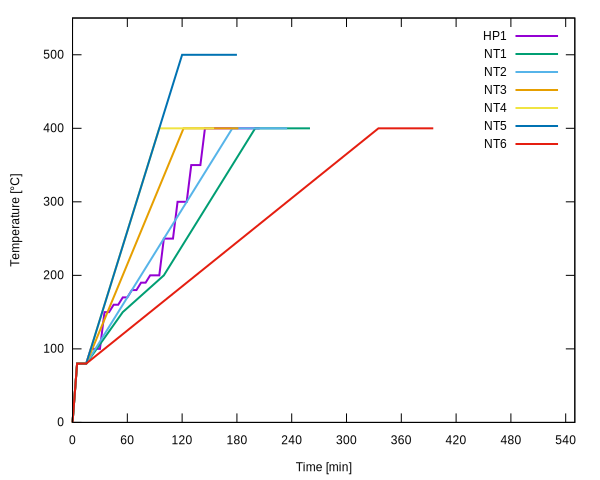
\includegraphics[width=.7\textwidth]{../Data/Graphs/hp1.png}
%	\caption{Different heatings curves}
%	\label{fig:heat}
%\end{figure}

%%%%%%%%%%%%%%%%%%%%%%%%%%%%%%%%%%%%%%%%%%%%%%%%%%%%%%%%%%%%%%%%%%%%%%%%%%%%%%%%%%%%%%%%
%%%%%%%%%%%%%%%%%%%%%%%%%%%%%%%%% CHARACTERISATION %%%%%%%%%%%%%%%%%%%%%%%%%%%%%%%%%%%%%
%%%%%%%%%%%%%%%%%%%%%%%%%%%%%%%%%%%%%%%%%%%%%%%%%%%%%%%%%%%%%%%%%%%%%%%%%%%%%%%%%%%%%%%%
\section{Characterisation}
All \gls{sem} micrographs were taken with a Zeiss Supra 40. 
\Gls{ft}\gls{uv}/\gls{vis}/\gls{nir} transmittance and reflectance spectra (at \SI{20}{\degree} incident 
angle) were recorded with a Bruker Vertex 70 
%transmission [\%] and reflection?  which angle? 
spectrometer with a quartz beam splitter, \SI{0.5}{\milli\meter} aperture and 
Gallium-Phosphide detector for ultra violet light (\SI{303}{\nano\meter}--\SI{588}
% gallium phosphide http://dx.doi.org/10.1051/epjconf/20134800028
{\nano\meter}) and a Silicon detector for visual and \gls{nir} light 
(\SI{500}{\nano\meter}--\SI{1.2}{\micro\meter}). For transmittance the light
entered the sample from the side with the layer. The \gls{uv} and \gls{vis}/\gls{nir} spectra were merged 
in Opus software. % included in the spectrometer. 
\Gls{xrd} spectra were obtained with a Thermo Scientific ARL Equinox 100 X-Ray Diffractometer. 
All \gls{xrd} spectra were taken at \SI{5}{\degree} incident angle and compared to the internal database.

The \gls{iv} curves were measured with Agilent 4156C Precision Semiconductor 
Parameter Analyzer from \SI{-0.5}{\volt} to \SI{0.5}{\volt} with steps of 
\SI{10}{\milli\volt}.
Prior to \gls{iv} measurements the samples were sputtered with aluminium 
through a mask to produce a multitude of equidistant contacts with a Leybold 
UNIVEX450C Sputter System.
Directional current sputtering was used with Argon as inert gas at \SI{0.005}{\milli\bar} 
and with a power of \SI{40}{\watt} for \SI{700}{\second}.
Between sputtering and \gls{iv} measurements 
direct contacts to the steel substrate were created by removing a patch of the \gls{zro}
layer with 
sand paper on two opposing edges of a sample and then by applying silver paste.
See figure~\ref{fig:circuit} for a sketch of the connectivity.

\begin{figure}[hbt]
    \centering
    \begin{circuitikz} \draw
        (0,0) to[european voltage source] (0,2)
        to[ammeter] (2,2) 
        to[generic,l=W] (4,2) 
        to[generic,l=Au] (6,2) 
        to[generic,l=Al] (8,2)
        -- (8,2)
        to[generic,l=ZrO$_2$] (8,0)
        -- (8,0)
        to[generic,l=steel] (6,0)
        to[generic,l=Ag] (4,0)
        to[generic,l=Au] (2,0) 
        to[generic,l=W] (0,0) 
            ;
    \end{circuitikz}
    \caption{Sketch of circuit, from the source clockwise: varibale voltage source, built-in amperometer, gold plated tungsten probe, sputtered aluminium contact, \gls{zro} layer to be measured, steel substrate, dried silver paste contact, gold plated tungsten probe.}
    \label{fig:circuit}
\end{figure}

%%%%%%%%%%%%%%%%%%%%%%%%%%%%%%%%%%%%%%%%%%%%%%%%%%%%%%%%%%%%%%%%%%%%%%%%%%%%%%%%%%%%%%%%
%%%%%%%%%%%%%%%%%%%%%%%%%%%%%%%%%%% PREOPTIMISATION %%%%%%%%%%%%%%%%%%%%%%%%%%%%%%%%%%%%
%%%%%%%%%%%%%%%%%%%%%%%%%%%%%%%%%%%%%%%%%%%%%%%%%%%%%%%%%%%%%%%%%%%%%%%%%%%%%%%%%%%%%%%%
\section{Pre-optimisation}\label{sec:exp-preopt}
%\td{the choice of grenzen for \gls{doe} was done by biotic reinforcement learning (i.e. my brain)}
%\td{Screening}
%The main part of the screening pre-optimisation samples were optimized via biotic reinforcement learning (i.e. my brain). 
The main part of all samples (around 90\%) were pre-optimization samples, 
from which the bulk were screening experiments optimized via biotic reinforcement learning 
(i.e. my brain) in order to obtain reasonable constraints for computerized pre-optimization. 
%Initially, glass plates were doctor bladed manually with aquatic solution and calcinated 
%via HP1. 
%Glass was used because of its availability and in order to be able to make IR 
%\td{transmission} spectra.
%In order to measure the resistivity of the produced layer \gls{fto} and \gls{ito} layered 
%glass plates (both conductive) were used as substrate.
%Conducting substrates were also needed to produce \gls{sem} micrographs. 
%\td{should maybe put this into beginning of section \ref{sec:exp}?}
%otherwise the sample would charge and can't be pictured anymore. 
%this means if the produced layer is thick and homogeneous enough, it's difficult to see in sem
%Different additives were included in the recipe (see table \ref{tab:rec1}) and the resistance was checked with a multimeter. 
%\todo{different additives, heating programs (NT1-NT5 and HP1), blade distances (distance between blade and substrate) and layer counts were tried}
Composition of the aquatic solution, heating program, blade distance (distance between 
blade and substrate) and layer count were varied but no homogeneous layers resulted. 
Thus, 
the buthanolic recipe was introduced, which gave rise to homogeneous films.
After the blade moved over the substrate the remaining liquid needed about a minute 
to evaporate. 
%\td{
The then current procedure resulted in clear and continuous films, but was plagued from 
inhomogeneities due to drying stains. 
The drying stains could be circumvented by using a heat gun, but the results were not 
reproducible. 
The glass plate of the film applicator was therefore exchanged with a metal plate which 
allowed to hold the sample in place through underpressure and simultaneously heat it to a certain 
temperature. The bounds of the process variables were then explored in a preliminary study 
using the Plackett-Burman\cite{Plackett1946} design implemented in the \texttt{python3} 
library \texttt{pyDOE}. With 
(1,5), (4,10), (400,500), (120,480), (0.1,5) and  (20,80) 
as nominal and extreme values for 
relative concentration of Zr $c_{zr}$, number of layers $\lambda$, calcination temperature $T_{cal}$[\oc{}], heating rate $v_{cal}$[\oc{}/\h{}], \gls{db} velocity $v_{DB}$[\mm{}/\s{}] and \gls{db} temperature $T_{DB}$[\oc{}], respectively. 
After testing the first samples, the lower limit for \gls{db} velocities was altered from 0.1 to 1 (see table \ref{tab:pre-opt1}).
\begin{table}[hbt]
	\centering
	\caption{Pre-optimization experiments}
	\label{tab:pre-opt}
	\begin{subtable}{0.5\linewidth}
		\centering
		\subcaption{Placket-Burman style experiments}
		\label{tab:pre-opt1}
		\begin{tabular}{cccccc}
			\hline
			\hline
	%		&80-150\oc{} [\oc{}/\minutes{}]	&150-200\oc{} [\oc{}/\minutes{}]	&200\oc{}-T$_{\textrm{Cal}}$ [\oc{}/\minutes{}]	&T$_{\textrm{Cal}}$ [\oc{}] &t$_{\textrm{Cal}}$ [\minutes{}]	\\
			$c_{zr}$	&$\lambda$	&$v_{DB}$	&$T_{DB}$	&$v_{cal}$	&$T_{cal}$		\\
			\hline
	1	&10	&5	&20	&120	&400	\\
	1	&4	&0.1	&20	&120	&500	\\
	5	&10	&0.1	&20	&120	&500	\\
	5	&4	&5	&20	&480	&400	\\
	1	&5	&5	&80	&120	&500	\\
	1	&10	&1	&80	&480	&400	\\
	5	&5	&1	&80	&120	&400	\\
	5	&10	&5	&80	&480	&500	\\
			\hline\hline
		\end{tabular}
	\end{subtable}%
	\begin{subtable}{0.5\linewidth}
		\centering
        \subcaption{Hand picked experiments; $^*$varied stabilisation agent}
		\label{tab:pre-opt2}
		\begin{tabular}{cccccc}
	%conc	&layers	&vDOC	&TDOC	&vCal	&Tcal		\\
			\hline\hline
			$c_{zr}$	&$\lambda$	&$v_{DB}$	&$T_{DB}$	&$v_{cal}$	&$T_{cal}$		\\
	%conc	&layers	&$v_{\textrm{DB}}$	&$T_{\textrm{DB}}$	&$v_{\textrm{cal}}$	&$T_{\textrm{cal}}$		\\
			\hline
	2	&8	&0.5	&40	&360	&470	\\
	2	&6	&2	&40	&360	&430	\\
	1	&4	&12	&70	&120	&500	\\
	1	&9	&18	&80	&240	&400	\\
	4$^*$	&6	&14	&60	&240	&500	\\
%	4$^\dagger$	&6	&14	&60	&240	&500	\\
%	4$^\ddagger$	&6	&14	&60	&240	&500	\\
			\hline
			\hline
			\\ \\  \\
%			\multicolumn{6}{c}{*different stabilisation reagent compositions}\\
		\end{tabular}
	\end{subtable}
\end{table}

%$T_{DB}$[\oc{}]
%$v_{DB}$[\mm{}/\s{}]
%$T_{cal}$[\oc{}]
%$v_{cal}$[\oc{}/\h{}]
%Especially the doctor blading velocity.
%}
%It was tried to reduce the waiting time and the resulting \td{drying stains}
%by using a heat gun. The drying was
%accelerated but not reproducibly and the glass plate on the film applicator was changed 
%against the heatable plate.
%With this new buthanolic recipe and heatable plate the limits of the optimization problem 
%were explored in a preliminary study using the Plackett-Burman \cite{Plackett1946} design 
%implemented in the \texttt{python3} library \texttt{pyDOE}.
%For the preliminary study a DB machine and NT were used and the steel. 
\ds{In the preliminary study only steel was used as substrate.}
%The Plackett-Burman \cite{Plackett1946} design implemented in the python3 library \texttt{pyDOE} was used to
%get an overview of reasonable boundaries.
%Latin squares were used to chose which experiments should be ausgefuehrt to get an ueberblick of the optimization room.
%See Code/Input_DOE/make_*exps.py and Code/Input_DOE/mail_theo
Some additional hand picked experiments (see table \ref{tab:pre-opt2}) were introduced to further narrow down the limits of 
the optimization as every reduction in variables or levels meant a faster convergence.
%ooooh 
%%%%%%%%%%%%%%%%%%%%%%%%%%%%%%%%%%%%%%%%%%%%%%%%%%%%%%%%%%%%%%
Shortly before the \gls{pso} the stabilisation agent was changed from \gls{acoh} to 
\gls{ipo} because of much better solution stability.
The - up to this moment - best process was chosen to be tested with 
\ml{1} \gls{acoh}, \ml{0.5} \gls{acoh} plus \ml{0.5} \gls{ipo} and \ml{1} \gls{ipo}.
%\td{As the sample showed the best all ex were proceeded with ipo as stabilisation agent. }
The sample produced with \gls{ipo} as stabilization agent 
showed comparable passivization results and better stability. 
Therefore \gls{ipo} was used  as stabilisation in further experiments.
After the boundaries of the solution were fixed 
the process variables to produce an insulating layer was examined. 
%There were many variables which had to be taken into account. 
%\td{plachett-burman design of experiment with conc, layers, calcination temperature, heating rate, DB velocity and DB temperature as input variables.}
See table \ref{tab:space} for the space spanned for the optimisation.
\begin{table}[ht!]
	\centering
	\caption{Final values used in the \gls{pso}.}
    \label{tab:space}
    \begin{tabular}{cccccc}
        \hline\hline
		$c_{zr}$	&$\lambda$	&$v_{DB}$	&$T_{DB}$	&$v_{cal}$	&$T_{cal}$		\\
%        concentration   &layers &\gls{db} velocity  &\gls{db} temperature   &heating rate   &calcination temperature    \\
        \hline
        2   &4  &10 &40 &120    &300    \\
        3   &6  &12 &50 &360    &400    \\
        4   &8  &14 &60 &600    &500    \\
        5   &10 &16 &70 &840    &       \\
            &12 &18 &80 &1080   &       \\
            &   &20 &   &       &       \\
        \hline\hline
    \end{tabular}
\end{table}

\ds{The final boundaries were
conc 2 - 5 (1) ,
layers 4 - 12 (2),
\gls{db} velocity 10 - 20 (2),
\gls{db} temperature 20 - 80 (20),
heating rate 120 - 1080 (240),
calcination temp 300 - 500 (100),
.
}

